
%(BEGIN_QUESTION)
% Copyright 2016, Tony R. Kuphaldt, released under the Creative Commons Attribution License (v 1.0)
% This means you may do almost anything with this work of mine, so long as you give me proper credit

\noindent
{\bf Lab Exercise -- introduction}

\vskip 5pt

Your task is to install an electronic ``smart'' positioner on a control valve, and control the position of that valve from the output of a single ``Hand Indicating Controller'' (HIC) in its ``manual'' mode.  Each instrument in the loop should be labeled with a proper tag name (e.g. ``HV-78'' for a hand-controlled valve), with all instruments in each loop sharing the same loop number.  Write on pieces of masking tape to make simple labels for all the instruments and signal lines.

The following table of objectives show what you and your team must complete within the scheduled time for this lab exercise.  Note how some of these objectives are individual, while others are for the team as a whole:

\underbar{Objective completion table:}

% No blank lines allowed between lines of an \halign structure!
% I use comments (%) instead, so that TeX doesn't choke.

$$\vbox{\offinterlineskip
\halign{\strut
\vrule \quad\hfil # \ \hfil & 
\vrule \quad\hfil # \ \hfil & 
\vrule \quad\hfil # \ \hfil & 
\vrule \quad\hfil # \ \hfil & 
\vrule \quad\hfil # \ \hfil & 
\vrule \quad\hfil # \ \hfil & 
\vrule \quad\hfil # \ \hfil \vrule \cr
\noalign{\hrule}
%
% First row
{\bf Performance objective} & {\bf Grading} & {\bf 1} & {\bf 2} & {\bf 3} & {\bf 4} & {\bf Team} \cr
%
\noalign{\hrule}
%
% Another row
Team meeting and prototype sketch (do {\it first!}) & mastery & -- & -- & -- & -- & \cr
%
\noalign{\hrule}
%
% Another row
Circuit design challenge & mastery & & & & & -- -- -- -- \cr
%
\noalign{\hrule}
%
% Another row
Final loop diagram and system inspection & mastery & & & & & -- -- -- -- \cr
%
\noalign{\hrule}
%
% Another row
Alignment of positioner to valve & mastery & -- & -- & -- & -- & \cr
%
\noalign{\hrule}
%
% Another row
Positioner calibration (with saturation) & mastery & -- & -- & -- & -- &  \cr
%
\noalign{\hrule}
%
% Another row
Demonstration of working system & mastery & -- & -- & -- & -- & \cr
%
\noalign{\hrule}
%
% Another row
Troubleshooting & mastery & & & & & -- -- -- -- \cr
%
\noalign{\hrule}
%
% Another row
Lab question: Instrument connections & proportional &  &  &  &  & -- -- -- -- \cr
%
\noalign{\hrule}
%
% Another row
Lab question: Commissioning & proportional &  &  &  &  & -- -- -- -- \cr
%
\noalign{\hrule}
%
% Another row
Lab question: Mental math & proportional &  &  &  &  & -- -- -- -- \cr
%
\noalign{\hrule}
%
% Another row
Lab question: Diagnostics & proportional &  &  &  &  & -- -- -- -- \cr
%
\noalign{\hrule}
%
% Another row
Decommissioning of positioners & mastery & -- & -- & -- & -- &  \cr
%
\noalign{\hrule}
} % End of \halign 
}$$ % End of \vbox

The only ``proportional'' scoring in this activity are the lab questions, which are answered by each student individually.  A listing of potential lab questions are shown at the end of this worksheet question.  The lab questions are intended to guide your labwork as much as they are intended to measure your comprehension, and as such the instructor may ask these questions of your team day by day, rather than all at once (on a single day).

%\vskip 10pt

{\bf It is essential that your team plans ahead what to accomplish each day.  A short (10 minute) team meeting at the beginning of each lab session is a good way to do this, reviewing what's already been done, what's left to do, and what assessments you should be ready for.  There is a lot of work involved with building, documenting, and troubleshooting these working instrument systems!}

As you and your team work on this system, you will invariably encounter problems.  You should always attempt to solve these problems as a team before requesting instructor assistance.  If you still require instructor assistance, write your team's color on the lab whiteboard with a brief description of what you need help on.  The instructor will meet with each team in order they appear on the whiteboard to address these problems.

$$\includegraphics[width=15.5cm]{i02590x01.eps}$$





\vfil \eject

\noindent
{\bf Lab Exercise -- team meeting, prototype sketch, and instrument selection}

\vskip 5pt

An important first step in completing this lab exercise is to {\bf meet with your instructor} as a team to discuss safety concerns, team performance, and specific roles for team members.  If you would like to emphasize exposure to certain equipment (e.g. use a particular type of control system, certain power tools), techniques (e.g. fabrication), or tasks to improve your skill set, this is the time to make requests of your team so that your learning during this project will be maximized.

\vskip 10pt

An absolutely essential step in completing this lab exercise is to work together as a team to {\bf sketch a prototype diagram} showing what you intend to build.  This usually takes the form of a simple electrical schematic and/or loop diagram showing all electrical connections between components, as well as any tubing or piping for fluids.  This prototype sketch need not be exhaustive in detail, but it does need to show enough detail for the instructor to determine if all components will be correctly connected for their safe function.

For example, if you intend to connect field devices to a PLC (Programmable Logic Controller), your prototype sketch must show how those devices will connect to typical input/output terminals on the PLC, where electrical power will be supplied, etc.  Prototype sketches need not show all intermediary connections between components, such as terminal blocks in junction boxes between the field device and the controller.

You should practice good problem-solving techniques when creating your prototype sketch, such as consulting equipment manuals for information on component functions and marking directions of electric current, voltage polarities, and identifying electrical sources/loads.  Use this task as an opportunity to strengthen your analytical skills!  Remember that you will be challenged in this program to do all of this on your own (during ``capstone'' assessments), so do not make the mistake of relying on your teammates to figure this out for you -- instead, treat this as a problem {\it you} must solve and compare your results with those of your teammates.

\vskip 10pt

You team will need to install a digital electronic (``smart'') positioner on the control valve you formerly ``rebuilt''.  The Fisher DVC series of electronic valve positioners is highly recommended for this lab exercise.

Consult documentation from the manufacturer's website to identify how to properly wire, power, and calibrate the transmitter.  Your instructor will check to see you have located and are familiar with the equipment manual(s).

The control valve should have mounting holes on its actuator assembly for receiving a positioner bracket.  This metal bracket will serve as the mounting ``platform'' for the positioner once attached to the valve actuator.  Brackets and positioners are not universal in design -- that is, they are made to match each other.

\vskip 10pt

{\bf A detail important for both safety and time management is to make sure you do not disturb the coupling of the valve body and actuator stems when connecting the positioner to the stem.}  On Fisher sliding-stem valves, particularly, the stem connector bolts must be un-done to attach the positioner's feedback linkage.  If the stem connector is loosened with full spring force applied to the valve seat (as is the case with any sliding-stem, air-to-open valve when no air pressure is applied), the actuator stem will slip loose and suddenly shift.  This will not only hurt your fingers if they are in the way of the actuator stem when it slips, but it will also necessitate a re-setting of the coupling between the valve body and actuator stems which can be time-consuming.

{\bf To avoid this problem on air-to-open valves, first apply enough air pressure to the actuator to raise the plug off the seat and relieve the seating force before loosening the stem coupling!}  With the valve plug held off the seat by air pressure, you may loosen the stem coupling with no risk of harm to yourself and little risk of disturbing the coupling position.

Another important detail regarding positioner installation is properly aligning the linkage between the positioner and the control valve stem.  Improper linkage alignment will result in non-linear valve travel (i.e. if 0\% and 100\% is accurate, 25\%, 50\% and/or 75\% will not be).  Again, consult the manufacturer's documentation for instructions on how to properly align the positioner-to-stem linkage.

\vskip 10pt

Positioners act as ``position controllers'' for control valves, sending enough air pressure as necessary to move the valve to match the signal given by the controller's output.  As controllers in their own right, positioners require a supply of compressed air to ``power'' them.  This air supply often needs to be of a different (greater) pressure than the air supply of an I/P signal converter.  For piston-actuated valves, the positioner often runs on 100 PSI compressed air, while the I/P converter runs on only 20 PSI.  As always, consult the manufacturer's manual for air supply specifications.

\vskip 10pt

{\bf Common mistakes:}

\begin{itemize}
\item{} Not checking valve stroke length for proper configuration before installing the positioner.
\item{} Disturbing the valve body/actuator stem coupling by disassembling the coupling when the actuator spring pressure is still seating the plug.
\item{} Incorrect installation and/or alignment of the linkage coupling the positioner to the valve stem: {\it consult the manual when installing your team's positioner to see exactly how it should attach!}
\item{} Improper pipe/tube fitting installation (e.g. trying to thread tube fittings into pipe fittings and vice-versa).
\end{itemize}




\vfil \eject

\noindent
{\bf Lab Exercise -- calibrating the positioner}

\vskip 5pt

When finished installing the positioner, you should test it prior to building the rest of the loop system.  Simply simulate the output signal of a loop controller by using a 4-20 mA loop calibrator in ``source'' mode, driving a signal to the I/P (or to the positioner directly, depending on the model) to stroke the valve.  

$$\includegraphics[width=15.5cm]{i02590x02.eps}$$

One of the criteria for a successful positioner calibration is that the positioner must ``saturate'' its output pressure(s) when the valve reaches full stroke.  For example, on a simple air-to-open valve calibration (i.e. 4 mA = valve at 0\% position ; 20 mA = valve at 100\% position), the positioner should saturate at beyond bench-set pressure at full signal (20 mA) and saturate at 0 PSI at minimum signal (4 mA) to ensure full seat loading.  This requirement is in addition to accurate positioning at all points between 0\% and 100\%.


\vskip 10pt

{\bf Common mistakes:}

\begin{itemize}
\item{} Incorrect supply pressure given to positioner
\end{itemize}


\vskip 10pt

{\bf Installing and roughly calibrating a positioner should take no more than one full lab session (3 hours) if all components are readily available and the team is working efficiently!}





\vfil \eject

\noindent
{\bf Lab Exercise -- circuit design challenge}

\vskip 5pt

Connect a loop-powered ``smart'' differential pressure transmitter (4-20 mA output with HART communication ability) to a DC voltage source and a meter such that the meter will indicate a increasing signal when a certain stimulus is applied to the transmitter, setting the transmitter's pressure measurement range as specified by the instructor.  All electrical connections must be made using a terminal strip (no twisted wires, crimp splices, wire nuts, spring clips, or ``alligator'' clips permitted).  You are expected to supply your own tools and multimeter.

This exercise tests your ability to navigate a ``smart'' instrument's parameters using a communicator as well as properly interpret terminal connections on a field instrument for signal and power.

$$\includegraphics[width=15.5cm]{i02590x03.eps}$$

\vskip 10pt

The following components and materials will be available to you: assorted 2-wire 4-20 mA differential pressure {\bf transmitters} calibrated to ranges 0-30 PSI or less, equipped with Swagelok compression tube connectors at the ``high'' and ``low'' ports ; lengths of {\bf plastic tube} with ferrules pre-swaged ; {\bf terminal strips} ; lengths of {\bf hook-up wire} ; 250 $\Omega$ (or approximate) {\bf resistors} ; analog {\bf meters} ; {\bf battery clips} (holders); {\bf HART communicator}.

\vskip 10pt

\noindent
{\bf Transmitter range} (instructor chooses): \hskip 20pt LRV = \underbar{\hskip 50pt} \hskip 20pt URV = \underbar{\hskip 50pt}

\vskip 10pt

\noindent
{\bf Meter options} (instructor chooses): \hskip 20pt \underbar{\hskip 20pt} Voltmeter (1-5 VDC) \hskip 10pt {\it or} \hskip 10pt \underbar{\hskip 20pt} Ammeter (4-20 mA)

\vskip 10pt

\noindent
{\bf Signal increases with...} (instructor chooses): \hskip 20pt \underbar{\hskip 20pt} Positive pressure \hskip 10pt {\it or} \hskip 10pt \underbar{\hskip 20pt} Vacuum (suction)

\vskip 10pt

\vfil

Study reference: the ``Analog Electronic Instrumentation'' chapter of {\it Lessons In Industrial Instrumentation}, particularly the sections on loop-powered transmitters and current loop troubleshooting.  Also, the ``Basic Concept of HART'' subsection of the ``The HART Digital/Analog Hybrid Standard'' section of the ``Digital Data Acquisition and Networks'' chapter of the same book.







\vfil \eject

\noindent
{\bf Lab Exercise -- building the system}

\vskip 5pt

The Instrumentation lab is set up to facilitate the construction of working instrument ``loops,'' with over a dozen junction boxes, pre-pulled signal cables, and ``racks'' set up with 2-inch vertical pipes for mounting instruments.  The only wires you should need to install to build a working system are those connecting the field instrument to the nearest junction box, and then small ``jumper'' cables connecting different pre-installed cables together within intermediate junction boxes.

After getting your prototype sketch approved by the instructor, you are cleared to begin building the positioner-equipped valve system.  This will consist of a loop controller placed into ``manual'' mode to allow direct control over the position of your team's valve as well as the valve of one more team.  

There will be no transmitter installed in this loop.  Feel free to use 1/4 inch plastic tubing for all pneumatic signal connections, and be sure not to exceed the rated supply pressure for the positioner (as documented in the positioner manual).

Select a specific loop controller to act as a display indicator for your system.  Your instructor may choose the controller for your team, to ensure you learn more than one type of controller during the course of a quarter.  The controller itself should be labeled ``HC-'' or ``HIC-'' because it is a ``hand'' controller, allowing a human operator manual control over the valve's position. 

Finally, your hand valve system needs to have a loop number, so all instruments may be properly labeled.  This loop number needs to be unique, so that another team does not label their instruments and cables the same as yours.  

\vskip 10pt

{\bf Common mistakes:}

\begin{itemize}
\item{} Failing to tug on each and every wire where it terminates to ensure a mechanically sound connection.
\item{} Students working on portions of the system in isolation, not sharing with their teammates what they did and how.  It is important that the whole team learns all aspects of their system!
\end{itemize}

\vskip 10pt

{\bf Building a functioning system from two working valves should take no more than one full lab session (3 hours) if all components are readily available and the team is working efficiently!}





\vfil \eject

\noindent
{\bf Lab Exercise -- documenting the system}

\vskip 5pt

Each student must sketch their own {\it loop diagram} for their team's system, following proper ISA conventions.  Sample loop diagrams are shown in the next question in this worksheet.  These loop diagrams must be {\it comprehensive} and {\it detailed}, showing every wire connection, every cable, every terminal block, range points, etc.  The principle to keep in mind here is to make the loop diagram so complete and unambiguous that anyone can follow it to see what connects to what, even someone unfamiliar with industrial instrumentation.  In industry, loops are often constructed by contract personnel with limited understanding of how the system is supposed to function.  The loop diagrams they follow must be so complete that they will be able to connect everything properly without necessarily understanding how it is supposed to work.

Every instrument and every signal cable in your loop needs to be properly labeled with an ISA-standard tag number.  An easy way to do this is to wrap a short piece of masking tape around each cable (and placed on each instrument) then writing on that masking tape with a permanent marker.  Although no industry standard exists for labeling signal cables, a good recommendation is to label each two-wire cable with the tag number of the field instrument it goes to.  Thus, every length of two-wire cable in a hand valve circuit should be labeled ``HV-$x$'' (where ``$x$'' is the loop number).  

When your entire team is finished drafting your individual loop diagrams, call the instructor to do an inspection of the loop.  Here, the instructor will have students take turns going through the entire loop, with the other students checking their diagrams for errors and omissions along the way.  During this time the instructor will also inspect the quality of the installation, identifying problems such as frayed wires, improperly crimped terminals, poor cable routing, missing labels, lack of wire duct covers, etc.  The team must correct all identified errors in order to receive credit for their system.  

After successfully passing the inspection, each team member needs to place their loop diagram in the diagram holder located in the middle of the lab behind the main control panel.  When it comes time to troubleshoot another team's system, this is where you will go to find a loop diagram for that system!

\vskip 10pt

{\bf Common mistakes:}

\begin{itemize}
\item{} Forgetting to label all signal wires (see example loop diagrams).
\item{} Forgetting to label all field instruments with their own tag names (e.g. PT-83).
\item{} Forgetting to note all wire colors.
\item{} Forgetting to put your name on the loop diagram!
\item{} Basing your diagram off of a team-mate's diagram, rather than closely inspecting the system for yourself.
\item{} Not placing loop sheet instruments in the correct orientation (field instruments on the left, control room instruments on the right).
\end{itemize}

\vskip 10pt

{\bf Creating and inspecting accurate loop diagrams should take no more than one full lab session (3 hours) if the team is working efficiently!}







\vfil \eject

\noindent
{\bf Lab Exercise -- troubleshooting}

\vskip 5pt

The most challenging aspect of this lab exercise is {\it troubleshooting}, where you demonstrate your ability to logically isolate a problem in the system.  All troubleshooting is done on an individual basis (no team credit!), and must be done {\it on a system you did not help build}, so that you must rely on loop diagrams to find your way around the system instead of from your own memory of building it.

Each student is given a limited amount of time to identify both the general location and nature of the fault, logically justifying all diagnostic steps taken.  All troubleshooting activities will take place under direct instructor supervision to ensure students are working independently and efficiently. 

Failure to correctly identify both the general location and nature of the fault within the allotted time, and/or failing to demonstrate rational diagnostic procedure to the supervising instructor will disqualify the effort, in which case the student must re-try with a different fault.  Multiple re-tries are permitted with no reduction in grade.

A standard multimeter is the only test equipment allowed during the time limit.  No diagnostic circuit breaks are allowed except by instructor permission, and then only after correctly explaining what trouble this could cause in a real system.  

The instructor will review each troubleshooting effort after completion, highlighting good and bad points for the purpose of learning.  Troubleshooting is a skill born of practice and failure, so do not be disappointed in yourself if you must make multiple attempts to pass!  One of the important life-lessons embedded in this activity is how to deal with failure, because it {\it will} eventually happen to you on the job!  There is no dishonor in failing to properly diagnose a fault after doing your level best.  The only dishonor is in taking shortcuts or in giving up.

\vskip 10pt

{\bf Common mistakes:}

\begin{itemize}
\item{} Neglecting to take measurements with your multimeter.
\item{} Neglecting to monitor pressure gauges on both positioners while testing the system.
\item{} Incorrectly interpreting the loop diagram (e.g. thinking you're at the wrong place in the system when taking measurements).
\item{} Incorrect multimeter usage (e.g. AC rather than DC, wrong range, wrong test lead placement).  This is especially true when a student comes to lab unprepared and must borrow someone else's meter that is different from theirs!
\end{itemize}

\vskip 10pt

{\bf Remember that the purpose of the troubleshooting exercise is to foster and assess your ability to intelligently diagnose a complex system.  Finding the fault by luck, or by trial-and-error inspection, is not a successful demonstration of skill.  The only thing that counts as competence is your demonstrated ability to logically analyze and isolate the problem, correctly explaining all your steps!}

\vskip 10pt

{\bf Troubleshooting takes a lot of lab time, usually at least two 3-hour lab sessions for everyone in a full class to successfully pass.  Be sure your team budgets for this amount of time as you plan your work, and also be sure to take advantage of your freedom to observe others as they troubleshoot, to better learn this art.}



\vfil \eject

\noindent
{\bf Lab questions}

\vskip 5pt

\begin{itemize}
\item{} {\bf Instrument connections}
\item{} Determine correct wire connections between instruments to create a working 4-20 mA loop circuit, based on diagrams of instruments with terminals labeled
\item{} Correctly determine all electrical sources and loads, as well as all voltage polarities and current directions in a 4-20 mA loop circuit, based on diagrams of instruments with terminals labeled
\end{itemize}

\filbreak

\begin{itemize}
\item{} {\bf Commissioning and Documentation}
\item{} Identify and explain the purpose of using a valve positioner on a pneumatic control valve
\item{} Explain how to properly align the linkage connecting the positioner to the valve stem, and why this alignment is important
\item{} Explain the significance of properly setting valve stroke length and bench-set pressure
\item{} Explain the function and purpose of the ``Out of Service'' mode on a Fisher DVC6000 series valve positioner
\item{} Explain how to isolate a control valve for removal and service using manual block and bypass valves
\item{} Identify some of the useful information obtained from a {\it valve signature} graph
\end{itemize}

\filbreak

\begin{itemize}
\item{} {\bf Mental math} (no calculator allowed!)
\item{} Calculate the flow coefficient (Cv) for a specific control valve given pressure drop and liquid flow rate
\item{} Calculate the liquid flow rate through a specific control valve given flow coefficient (Cv) and pressure drop
\item{} Calculate force generated by a diaphragm or piston actuator given diameter and applied fluid pressure in units of PSI
\end{itemize}

\filbreak

\begin{itemize}
\item{} {\bf Diagnostics}
\item{} Explain how to confirm the presence of an {\it open} in a 4-20 mA signal cable using only a voltmeter (no resistance or current measurement allowed!).
\item{} Explain how to confirm the presence of a {\it short} in a 4-20 mA signal cable using only a voltmeter (no resistance or current measurement allowed!)  
\item{} Determine whether or not a given diagnostic test will provide useful information, given a set of symptoms exhibited by a failed system
\item{} Identify at least two plausible faults given the results of a diagnostic test and a set of symptoms exhibited by a failed system
\item{} Propose a diagnostic test for troubleshooting a failed system and then explain the meanings of two different test results
\end{itemize}



\vfil \eject

\noindent
{\bf Lab Exercise -- decommissioning and clean-up}

\vskip 5pt

The final step of this lab exercise is to decommission your team's valve control loop and re-stock the smart positioner back to the proper storage location.  {\bf It is critically important to keep all the feedback hardware (connector arms, adjustment arms, etc.) with the positioner, ideally using tape to affix these parts to the positioner, or placing each positioner and feedback hardware into a container, so they do not become separated and lost.}  Remove your system documentation (e.g. loop diagram) from the common holding area, either discarding it or keeping it for your own records.  Also, remove instrument tag labels (e.g. FT-101) from instruments and from cables.  Perform general clean-up of your lab space, disposing of all trash, placing all tools back in their proper storage locations, sweeping up bits of wire off the floor and out of junction boxes, etc.

\vskip 10pt

\indent
{\bf Leave the following components in place, mounted on the racks:}

\begin{itemize}
\item{} Large control valves and positioners
\item{} I/P transducers
\item{} Large electric motors
\item{} Large variable-frequency drive (VFD) units
\item{} Cables inside conduit interconnecting junction boxes together
\item{} Pipe and tube fittings (do not unscrew pipe threads)
\item{} Supply air pressure regulators
\end{itemize}

\vskip 10pt

\indent
{\bf Return the following components to their proper storage locations:}

\begin{itemize}
\item{} Sensing elements (e.g. thermocouples, pH probes, etc.)
\item{} Process transmitters
\item{} ``Jumper'' cables used to connect terminal blocks within a single junction box
\item{} Plastic tubing and tube fittings (disconnect compression-style tube fittings)
\item{} Power cables and extension cords
\item{} Adjustment (loading station) air pressure regulators
\end{itemize}

\vskip 10pt

Finally, you shall return any control system components to their original (factory default) configurations.  This includes controller PID settings, function block programs, input signal ranges, etc.


\underbar{file i02590}
%(END_QUESTION)





%(BEGIN_ANSWER)


%(END_ANSWER)





%(BEGIN_NOTES)

\noindent
{\bf Loop diagrams / inspections:}

I strongly recommend checking off students' loop diagrams while you inspect their loop (checking for secure wiring, proper tubing, good conduit installation, etc.) with them.  Have all team members take you on a ``tour'' of their completed loop, with each team member explaining a different portion of the loop you select while using their own loop diagram as a guide.  While a student is explaining their section of the loop, you can check the other students' loop diagrams for accuracy.  This not only saves time by consolidating the tasks of loop inspection and loop diagram verification, but it also ensures students can actually relate their loop diagrams to the loop they have built and articulate that understanding to you.

\vskip 10pt

\goodbreak

\noindent
{\bf Troubleshooting fault ideas:}

\begin{itemize}
\goodbreak
\item{} Connect instrument tubes to wrong port (construction fault)
\item{} Replace I/P restrictor with pre-faulted (plugged) unit (high output fault)
\item{} Replace I/P relay with pre-faulted unit (low or high output fault)
\item{} Turn supply air pressure down well below 15 PSI (low output fault)
\item{} Strip wire at terminal, then insert insulated wire end under terminal and tighten (open wire fault)
\item{} Cut signal cable somewhere in mid-conduit (open wire fault)
\item{} Push a thumbtack through the cable somewhere in mid-conduit (shorted wire fault)
\item{} Wire instrument cable conductors backward (construction fault)
\item{} Configure transmitter for excessive damping (slow response fault)
\item{} Configure indicator/controller for excessive damping (slow response fault)
\item{} Miscalibrate transmitter and/or indicator/controller (inaccuracy fault)
\item{} Plug tube connections using portion of foam earplug stuffed into tube fitting (slow response fault)
\item{} Reverse action of controller/positioner/transmitter (wrong response fault)
\item{} Mis-configure linear/sq.root characterization of transmitter and/or indicator/controller (nonlinearity fault)
\item{} Connect 2.2 k resistor in parallel with 4-20 mA transmitter to simulate partial short in wiring (inaccuracy fault)
\item{} Exchange 250 ohm resistor for a different resistor that looks the same but has the wrong value (inaccuracy fault) 
\item{} Unplug cable(s) inside transmitter or controller (failed instrument fault)
\item{} Give students wrong loop diagram (documentation fault)
\item{} Start students out on wrong controller (operator error)
\item{} Close valve and leave safety tag hanging on it (operator/technician error)
\end{itemize}









\vfil \eject

\noindent
{\bf Lab questions}

\vskip 20pt

\item{$(1)$} Explain the technology used by your team's electronic positioner to sense the control valve stem's position, and identify ways in which this feedback sensor could possibly fail.

\vskip 20pt

\item{$(2)$} Explain the function and purpose of the ``Out of Service'' mode on a Fisher DVC6000 series valve positioner.

\vskip 20pt

\item{$(3)$} Calculate the flow coefficient ($C_v$) for a control valve with a pressure drop of 49 PSID and a water flow rate of 400 gallons per minute.

\vskip 20pt

\item{$(4)$} Control valve HV-1a remains shut all the time, while valve HV-1b remains wide-open, no matter the output value of controller HIC-1.  Identify one possible fault, as well as one impossible fault, with regard to these symptoms.  Be specific in your identification: both the location (which component) and nature (e.g. open, shorted, plugged) of each fault. 

$$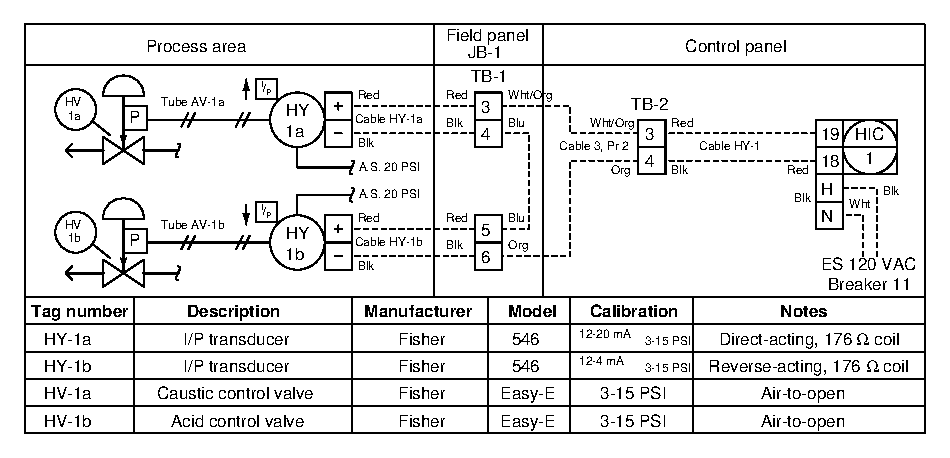
\includegraphics[width=15.5cm]{i02590x04.eps}$$


%INDEX% Lab exercise, electronic valve positioner

%(END_NOTES)


